% % !TEX root = main.tex
% \documentclass[journal]{IEEEtran}
% \input{tip_shared}
% \allowdisplaybreaks[2]

% % 跨文档引用配置
% \usepackage{xr-hyper}  % 推荐使用 xr-hyper（支持hyperref）
% \usepackage{hyperref}  % 如果需要超链接支持

% \externaldocument{main}  

This supplementary material provides detailed experimental settings and additional results.

% In \Cref{Appendix: Preliminaries and notations}, we give some basic definitions and lemmas for the following analysis.

% In \Cref{Appendix: main proofs}, we discuss the main assumptions.

% In \Cref{Appendix: Experiment details}, we provide the experimental details and additional experiments.

\section{Experiment Details}
\label{Appendix: Experiment details} 
\subsection{Deep Pairwise Supervised Hashing Formulation}
\label{Appendix: hashing formulation}

We consider deep supervised pairwise hashing in our experiments, which aims to learn binary codes that minimize Hamming distances for similar pairs and maximize them for dissimilar pairs. Let $\bA = \{\ba_i \in \RR^{d_a} : i = 1, \ldots, n\}$ be the training set with labels $\calY = \{\by_i \in \{0,1\}^C\}$ (one-hot for single-label, multi-hot for multi-label). Key notations are in \Cref{Table:notations_for_deep_hashing}.


\paragraph{Network Architecture}  
A CNN extracts features from $\ba_i$, followed by a fully connected hash layer producing $d$-dimensional outputs $\bC(\bx; \ba_i)\blue{=:\bC_i(\bx)}$, which are passed through $\tanh$ to yield \blue{the continuous codes $\bD_i(\bx)=\tanh(\bC_i(\bx))$}.


\paragraph{Loss Function}  
For hash codes in $\{-1,1\}^d$, the Hamming distance is $d_{ij}^h = \tfrac{1}{2}(d - \langle \bh_i, \bh_j \rangle)$. Following \cite{xiaSupervisedHashingImage2014,laiSimultaneousFeatureLearning2015}, similarity $s^o_{ij} = 1$ if samples share labels, else $0$. The likelihood is:
\[
P(s^o_{ij} \mid \bh_i, \bh_j) = \blue{\operatorname{sig}_{\kappa}}(\langle \bh_i, \bh_j \rangle)^{s^o_{ij}} \left(1 - \blue{\operatorname{sig}_{\kappa}}(\langle \bh_i, \bh_j \rangle)\right)^{1 - s^o_{ij}},
\]
where $\blue{\operatorname{sig}_{\kappa}(t) = (1 + \exp(-\kappa t))^{-1}}$, $\blue{\kappa} < 1$. Using continuous codes $\blue{\bD_i(\bx)}$ and $s^h_{ij} = \tfrac{1}{2} \langle \blue{\bD_i(\bx), \bD_j(\bx)} \rangle$, the loss becomes:
\begin{align}
\label{Eq: the pairwise CE loss}
\min_{\bx} \; \blue{\ell_{\calS}}(\bx) = -\frac{1}{|\calS|} \sum_{s^o_{ij} \in \calS} \log\left(1 + \exp\left(-\blue{\kappa} s^o_{ij} s^h_{ij}\right)\right).
\end{align}

We use the W-type regularization:
\begin{align}
\label{Eq: the W-type regularization}
h(\bZ) = \sum_{i=1}^n h(\bz_i), \quad h(\bz) = \lambda \|\,|\bz| - \bm{1}\,\|_1,
\end{align}
where $\lambda > 0$ controls regularization strength.

Combining \eqref{Eq: the pairwise CE loss} and \eqref{Eq: the W-type regularization} into \eqref{Prop: block-wise regularized problem} gives the final loss of DualHash in our experiments.
\begin{align}
% \label{Eq: the pairwise quantization-based hashing}
\min_{\bx \in \calX, \bB \in \RR^{n\times d}} \; 
&-\frac{1}{|\calS|} \sum_{s^o_{ij} \in \calS} \log\left(1 + \exp\left(-\blue{\kappa} s^o_{ij} s^h_{ij}\right)\right) \notag \\
&+ \frac{\gamma}{2n}\sum_{i=1}^n \| \bb_i - \blue{\bD_i(\bx)}\|_2^2 
+ \sum_{i=1}^n \lambda \|\,|\bb_i| - \bm{1}\,\|_1. \notag
\end{align}


\paragraph{Out-of-sample Extension}  
For an unseen query $\blue{\ba^{\mathrm{qry}}} \notin \bA$, its binary code is predicted as:
\[
\blue{\bh^{\mathrm{qry}}} = \operatorname{sgn}(\bC(\bx; \blue{\ba^{\mathrm{qry}}})).
\]

\subsection{Implementation Details}
\label{Appendix: Details of experiment implementation}
\begin{table}[thbp]
    \centering
    \caption{Summary of symbols and notations.}
    \label{Table:notations_for_deep_hashing}
    \small
    \begin{tabular}{ll}
        \toprule 
        \textbf{Symbol} & \textbf{Description} \\
        \midrule 
        $\ba_{i}$, $\by_{i}$ & Input feature and label vector for \\
                             & $i$-th sample \\
        $s_{ij}^{o}$, $s_{ij}^{h}$ & Similarity in input space and \\
                                   & Hamming space \\
        $d_{ij}^{o}$, $d_{ij}^{h}$ & Distance in input space and \\
                                   & Hamming space \\
        $\bC(\bx; \ba_{i})$ & Network output before activation \\
        $\blue{\bh_{i}}\in \{-1, 1\}^{d}$ & Binary hash code for $i$-th sample \\
        \blue{$\bb_{i}\in \RR^{d}$} & \blue{Continuous auxiliary variable ($i$-th row of $\bB$)} \\
        $\blue{\bD_{i}(\bx)}= \tanh(\bC(\bx; \ba_{i}))$ & Continuous code after activation \\
        $n$, $d$ & Number of samples and hash \\
                 & code length \\
        $\bx$ & Network parameters \\
        $d_{\ba}$, $\blue{q}$ & Dimension of input feature and \\
                           & parameters \\
        \bottomrule
    \end{tabular}
\end{table}
\paragraph{Baseline methods}
We compare our method with eight baseline approaches, including one traditional discrete hashing method and seven deep supervised hashing methods:
\begin{enumerate}[label=(\roman{*}),leftmargin=2em]
    \item \textbf{SDH}~\cite{shenSupervisedDiscreteHashing2015}: A pointwise supervised hashing method using hand-crafted features. It employs discrete cyclic coordinate descent to directly optimize binary codes.
    
    \item \textbf{DHN}~\cite{zhuDeepHashingNetwork2016}: A Bayesian framework that minimizes pairwise cross-entropy loss and quantization error using $\tanh$ relaxation and $\sum_i\log(\cosh(|z_i|-1))$ regularization.
    
    \item \textbf{DSH}~\cite{liuDeepSupervisedHashing}: Uses max-min pairwise loss with $\||\bz|-\bm{1}\|_1$ regularization to minimize quantization error.
    
    \item \textbf{DTSH}~\cite{wang2016DTSH}: Learns hash codes by maximizing triplet likelihood with negative log-triplet loss, using  $\||\bz|-\bm{1}\|^2_2$  quantization regularization and a positive margin $\alpha$ to accelerate training and normalize Hamming distance gaps.
    
    \item \textbf{HashNet}~\cite{Cao2017HashNetDL}: Progressively increases $\beta$ in $\tanh(\beta x)$ to approximate the $\text{sgn}$ function, addressing nonconvex optimization challenges.
    
    \item \textbf{DSDH}~\cite{li2017deep}: Integrates pairwise labels and classification information using alternating minimization to learn features and binary codes with the $\text{sgn}$ function.
    
    \item \textbf{OrthoHash}~\cite{hoeOneLossAll2021}: Uses a single cosine similarity loss to maximize alignment between continuous codes and binary orthogonal codes, ensuring discriminativeness with minimal quantization error.
    
    \item \textbf{MDSHC}~\cite{wang2023deep}: A two-stage method that first generates hash centers with minimal Hamming distance constraints, then uses three-part losses with $\||\bz|-\bm{1}\|_1$ regularization to reduce quantization error.
\end{enumerate}


\paragraph{Evaluation Protocols}
Following \cite{liuDeepSupervisedHashing}, we adopt four evaluation metrics:

\begin{enumerate}[label=\textup{(\roman{*})}, leftmargin=2em]
    \item \textit{Mean Average Precision (mAP)}: For a query $\blue{\ba^{\mathrm{qry}}}$, the Average Precision is computed as:
    \[
        \text{AP}(\blue{\ba^{\mathrm{qry}}}) = \frac{\sum_{k=1}^{N} P(k) \cdot \mathbb{I}_{\text{rel}}(k)}{\min(N, \blue{R^{\mathrm{qry}}})},
    \]
    where $P(k)$ is precision at rank $k$, $\mathbb{I}_{\text{rel}}(k)$ indicates whether the $k$-th result is relevant, $\blue{R^{\mathrm{qry}}}$ is the total relevant samples, and $N$ is the number of retrieved items. mAP averages AP over all queries. For CIFAR-10, we use all returned neighbors; for NUS-WIDE, we consider top-5000 results.
    
    \item \textit{Precision at Top K (P@topK)}: The proportion of true neighbors among top-K retrieved results, averaged over all queries.
    
    \item \textit{Precision within Hamming Radius 2 (P@r=2)}: Measures retrieval accuracy for items within Hamming distance 2 from the query. This metric is particularly efficient as Hamming radius search has $\mathcal{O}(1)$ time complexity per query.
    
    \item \textit{Precision-recall curves of Hamming ranking}: PR curves illustrate
        precision at various levels of recall, offering insights into the trade-off between precision and recall at different thresholds. These curves are widely
        recognized as effective indicators of the robustness and overall performance
        of different algorithms.
\end{enumerate}

\section{Additional Experimental Results}
\subsection{Comparison of Optimization Algorithms with Different W-Type Regularizations}
To validate the effectiveness of our primal-dual framework, we compare DualHash-StoM
against optimization algorithms with different W-type regularizations. \Cref{tab:4_algorithms_for_hash_regularization_and_update}
summarizes the configurations of different regularization functions and their corresponding optimization approaches. For StoMHash-WCR, we employ the regularization $\lambda \| \bz^{2}- \mathbf{1}\|_1$
following the iSPALM framework \cite{InertialProximalAlternating}. The proximal
operator is computed with parameter $\rho > 0$ under the condition
$\frac{\rho}{\eta}> \frac{1}{2}$, which ensures the subproblem is strongly convex
with a unique solution.
% $$\text{prox}_{\rho f}(\bx) = \arg \min_{y}\left( \eta \|\by^{2}- \mathbf{1}\| + \frac{\rho}{2} \|\by - \bx\|^{2}\right).$$

\begin{table}[htbp]
    \centering
    \caption{Configurations of different W-type regularizations and optimization algorithms for DualHash-StoM and three baselines.}
    \label{tab:4_algorithms_for_hash_regularization_and_update}
    \resizebox{0.93\textwidth}{!}{
    \begin{tabular*}{1\textwidth}{@{\extracolsep{\fill}}lcccc@{}}
        \toprule 
        Method & $h(\bz)$ & Convexity & Algorithm & Complexity \\
        \midrule 
        DSH \cite{liuDeepSupervisedHashing} & $\| |\bz| - \mathbf{1}\|_{1}$ & Nonconvex & SGDM & -- \\
        StoMHash-WCR & $\| \bz^{2}- \mathbf{1}\|_{1}$ & Weakly convex & SPGD & -- \\
        DHN \cite{zhuDeepHashingNetwork2016} & $\sum_{i}\log(\cosh(|z_{i}| - 1))$ & Nonconvex & SGDM & -- \\
        \textbf{DualHash-StoM} & $\| |\bz| - \mathbf{1}\|_{1}$ & Nonconvex & PD & $\checkmark$ \\
        \bottomrule
    \end{tabular*}}
    \vspace{-3pt}
    \parbox{0.93\textwidth}{\footnotesize
    \textbf{Notes}: \textbf{Algorithm} describes the optimization strategy: SGDM (stochastic subgradient descent with momentum), SPGD (stochastic proximal gradient descent), PD (primal-dual). \textbf{Complexity} reports oracle complexity; `--' indicates no analysis available.
    }
\end{table}

\paragraph{Training performance analysis}
Figures \ref{Fig: Comparison of training performance of Different Methods on CIFAR-10} and \ref{Fig: Comparison of training performance of Different Methods on NUS-WIDE} present
training dynamics across different optimization approaches, comparing training loss, P@top1000, and P@r=2 metrics \textbf{for 64-bit codes} on CIFAR-10 and NUS-WIDE. On
CIFAR-10, DualHash-StoM demonstrates strong optimization efficiency across all
metrics. Our method achieves fast convergence in training loss while consistently maintaining high P@r=2 and P@top1000 values throughout the
optimization process. While StoMHash with weakly convex regularization (StoMHash-WCR)
shows competitive performance, DualHash-StoM achieves faster convergence
and higher retrieval performance, demonstrating the effectiveness of our
primal-dual transformation for handling W-type regularizations. On the more challenging NUS-WIDE dataset with complex multi-label scenarios, DualHash-StoM maintains
competitive retrieval performance despite slightly slower initial convergence.
The experimental results on diverse datasets indicate that
utilizing nonconvex nonsmooth regularization with specialized primal-dual
optimization can improve hash code learning and retrieval
performance in practical applications.

\begin{figure}[t]
    \centering
    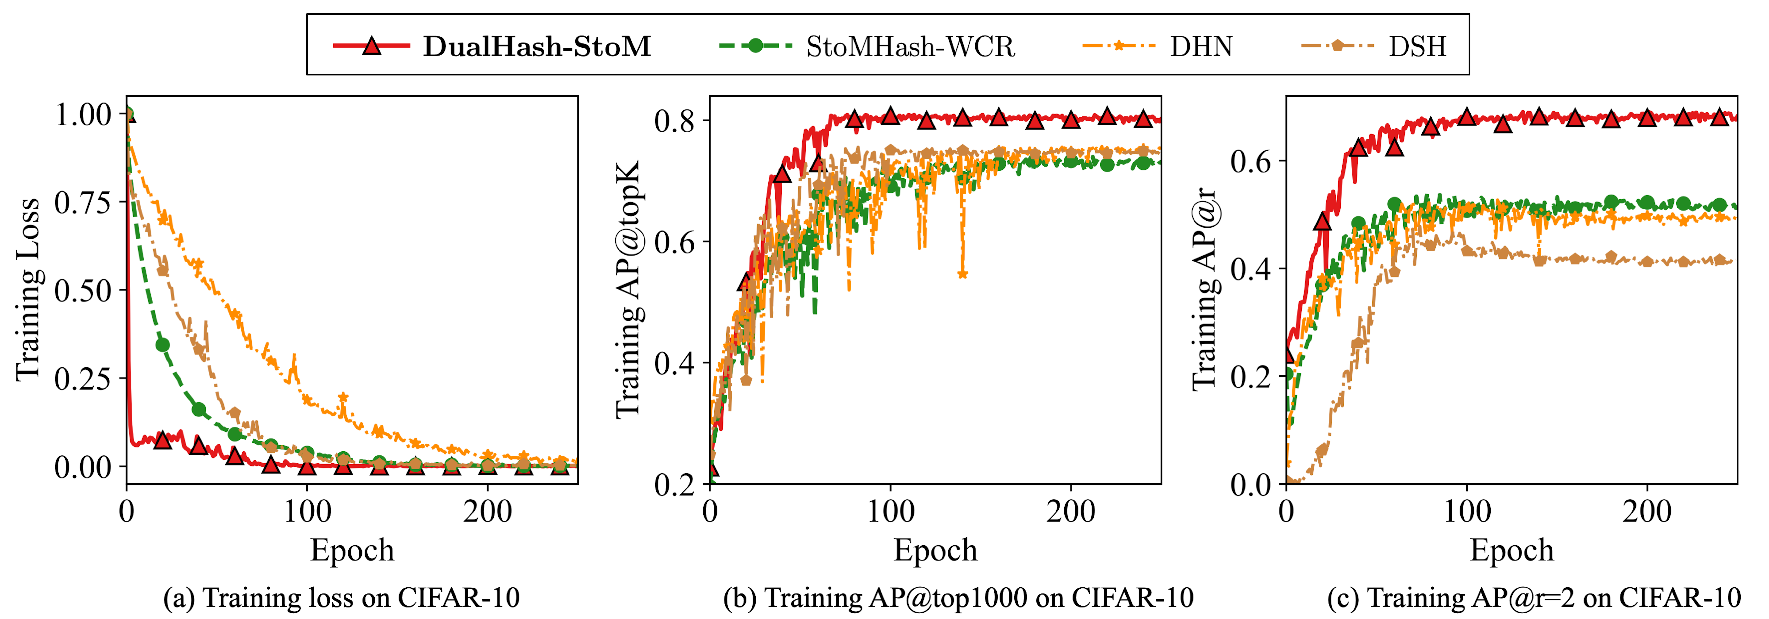
\includegraphics[width=0.95\textwidth]{results_images/ex3_training_cifar10.pdf}
    \caption{Training performance comparison of DualHash-StoM and three baselines with 64-bit codes on the CIFAR-10 dataset.}
    \label{Fig: Comparison of training performance of Different Methods on CIFAR-10}
\end{figure}
\begin{figure}[t]
    \centering
    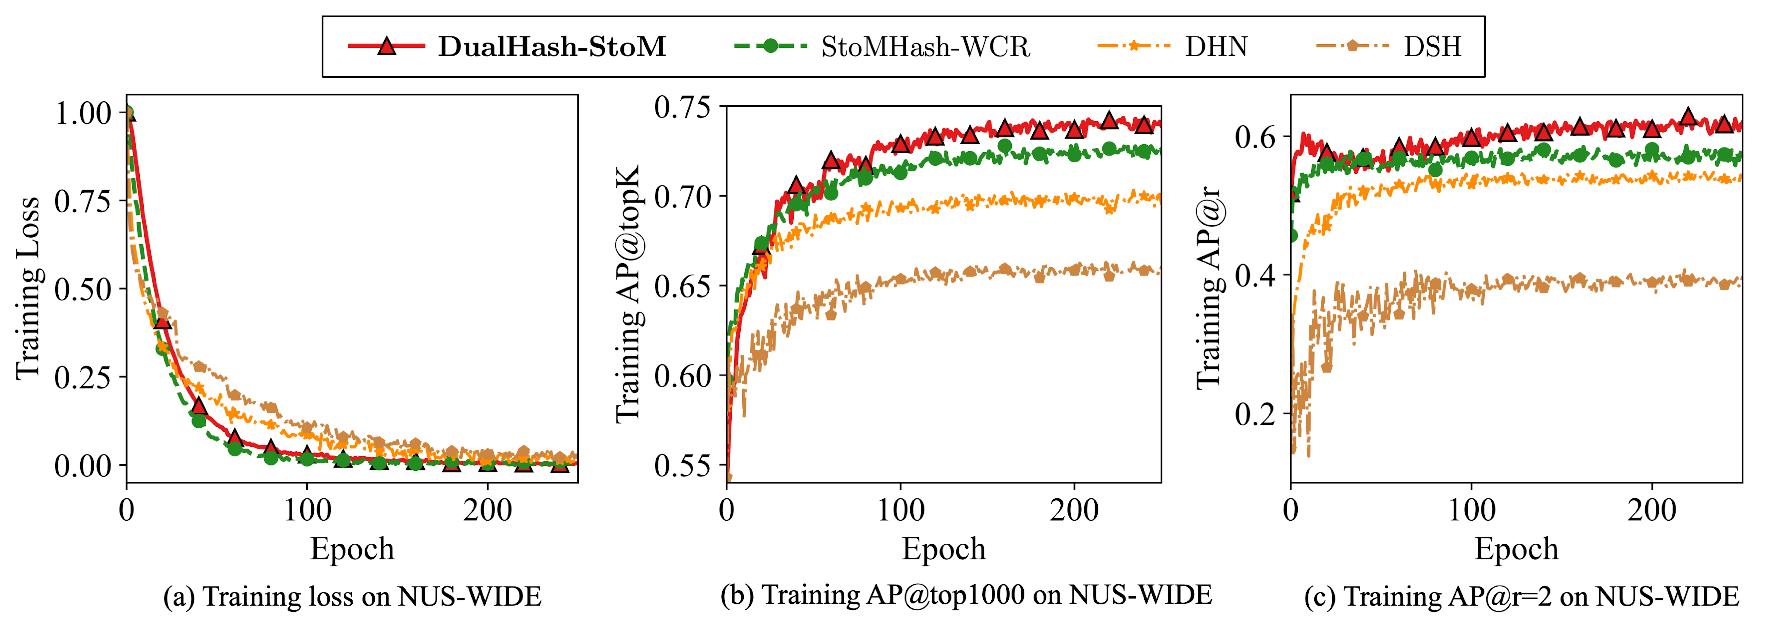
\includegraphics[width=0.95\textwidth]{results_images/ex3_training_nuswide.pdf}
    \caption{Training performance comparison of DualHash-StoM and three baselines with 64-bit codes on the NUS-WIDE dataset.}
    \label{Fig: Comparison of training performance of Different Methods on NUS-WIDE}
\end{figure}

\begin{table}[htbp]
    \centering
    \caption{Retrieval performance comparison of DualHash-StoM and three baselines with 64-bit codes on CIFAR-10 and NUS-WIDE datasets.}
    \label{tab:performance_comparison_64bits}
    \resizebox{0.93\textwidth}{!}{
    \begin{tabular*}{1\textwidth}{@{\extracolsep{\fill}}lcccccc@{}}
        \toprule 
        \multirow{2}{*}{Methods} & \multicolumn{3}{c}{CIFAR-10} & \multicolumn{3}{c}{NUS-WIDE} \\
        \cmidrule(lr){2-4} \cmidrule(lr){5-7}
         & mAP@All & P@r=2 & Time\textsuperscript{*} & mAP@5000 & P@r=2 & Time\textsuperscript{*} \\
        \midrule 
        DSH \cite{liuDeepSupervisedHashing} & 0.8010 & 0.4401 & 7.38 & 0.6634 & 0.4004 & 21.14 \\
        DHN \cite{zhuDeepHashingNetwork2016} & 0.8051 & 0.5272 & \textbf{6.74} & 0.7042 & 0.5432 & \textbf{16.47} \\
        StoMHash-WCR & 0.7773 & 0.5402 & 7.04 & 0.7225 & 0.5857 & 16.69 \\
        \textbf{DualHash-StoM} & \textbf{0.8539} & \textbf{0.6872} & 6.86 & \textbf{0.7448} & \textbf{0.6548} & 16.83 \\
        \bottomrule
    \end{tabular*}}
    
    \parbox{0.93\textwidth}{\footnotesize
    \textsuperscript{*}Training time per epoch (seconds). \textbf{Bold} values indicate the best results.
    }
\end{table}

\paragraph{Retrieval performance in Hamming space}
We report mAP, P@r=2, and the average time per training epoch on CIFAR-10 and NUS-WIDE, all
with 64-bit codes, for different methods in
Table~\ref{tab:performance_comparison_64bits}. The results highlight the superior retrieval
accuracy of DualHash-StoM compared to the baseline methods.

Specifically, on the CIFAR-10 dataset, DualHash-StoM achieves 9.9\% and 27.2\%
improvements over StoMHash-WCR in mAP@All and P@r=2, respectively. Similarly, on the
NUS-WIDE dataset, DualHash-StoM outperforms StoMHash-WCR with a 3.1\% improvement
in mAP@5000 and an 11.8\% improvement in P@r=2. Computationally, DualHash-StoM shows comparable efficiency to baselines such as DHN
(e.g., 6.86s vs. 6.74s on CIFAR-10 and 16.83s vs. 16.47s
on NUS-WIDE). This marginal time increase is justified by the substantial performance gains.
Furthermore, \Cref{fig:ex3_testing_2datasets} displays P@topK results and PR curves
with 64-bit codes on CIFAR-10 and NUS-WIDE. DualHash-StoM consistently outperforms all
comparison methods by large margins in P@topK. For PR curves, DualHash-StoM
demonstrates superior performance at lower recall levels, making it especially well-suited
for precision-critical image retrieval systems.

\begin{figure}[htbp]
    \centering
    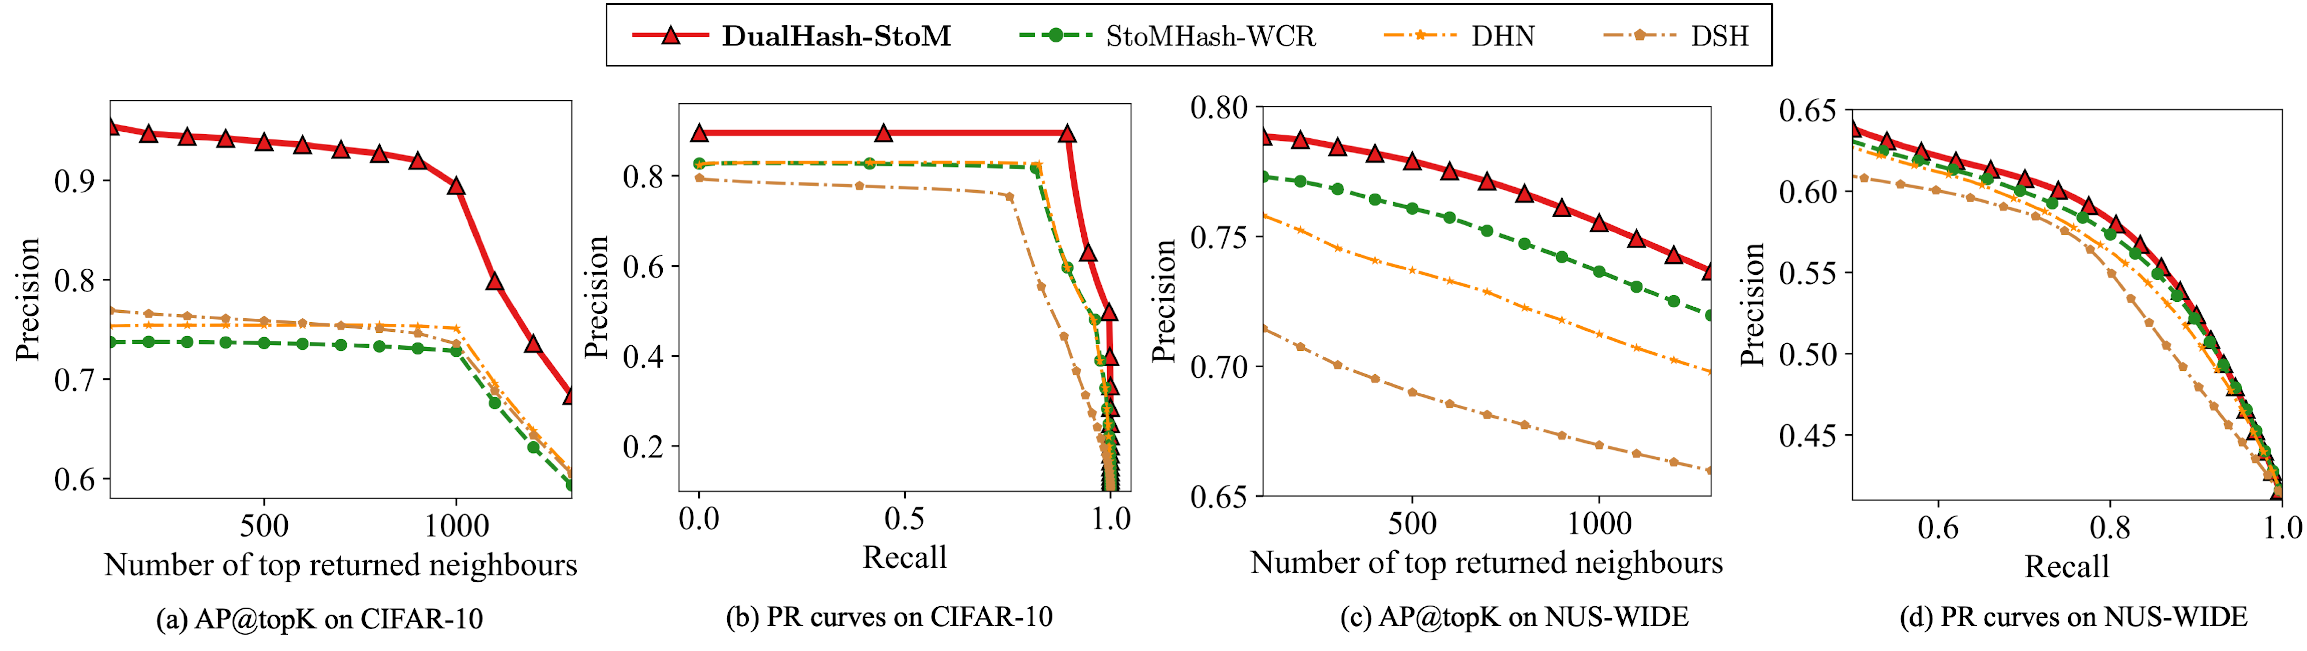
\includegraphics[width=0.95\textwidth]{results_images/ex3_testing_2datasets.pdf}
    \caption{Retrieval performance comparison of DualHash-StoM and three baselines with 64-bit codes on CIFAR-10 and NUS-WIDE datasets. (a), (c): P@topK results; (b), (d): PR curves.}
    \label{fig:ex3_testing_2datasets}
\end{figure}

% \end{document}
